\documentclass[12pt]{book}

\usepackage[swedish]{babel}	% För svensk avstavning och svenska rubriker (t ex "innehållsförteckning)
\usepackage{fontspec}

%\usepackage[scaled]{beramono}
%\setmonofont{Bera Mono}
\usepackage[T1]{fontenc}		% För svenska bokstäver
\DeclareTextCommand{\nobreakspace}{T1}{\leavevmode\nobreak\ }


\usepackage{titling}
\usepackage[left=2cm, right=2cm,bottom=2cm,top=1cm, paperwidth=297mm, paperheight=210mm, twoside=false]{geometry}

\usepackage{bookman}
\renewcommand{\familydefault}{\sfdefault}
%\usepackage{tgtermes} %times
\usepackage[scaled]{uarial} %Arial
\usepackage{sectsty}
\allsectionsfont{\sffamily}
\usepackage{inconsolata}
\addto\captionsswedish{%
\def\contentsname{Innehåll}}
\usepackage{url}
\usepackage{hyperref}
\usepackage{wrapfig}
\usepackage{graphicx}
\usepackage[usenames,dvipsnames]{xcolor}
\usepackage{array} %to center table cells
\usepackage{parskip} %to have noindent and space between paras

\usepackage{titlesec}
%\titleformat{\chapter}[hang]{\Huge\sffamily}{\thechapter.~}{0pt}{\Huge\sffamily}
\titleformat{\chapter}[hang]{\bf\fontsize{40}{40}\selectfont\centering\vskip-13mm}{}{0pt}{\bf\fontsize{40}{40}\selectfont}
\titleformat{\section}[hang]{\bf\fontsize{20}{20}\selectfont}{}{0pt}{\bf\fontsize{20}{20}\selectfont}

\usepackage{multicol}

\usepackage{listings}
% "define" Scala
\lstdefinelanguage{scala}{
  morekeywords={abstract,case,catch,class,def,%
    do,else,extends,false,final,finally,%
    for,forSome,if,implicit,import,lazy,match,%
    new,null,object,override,package,%
    private,protected,return,sealed,%
    super,this,throw,trait,true,try,%
    type,val,var,while,with,yield},
  otherkeywords={=>,<-,<\%,<:,>:,@},
  sensitive=true,
  morecomment=[l]{//},
  morecomment=[n]{/*}{*/},
  morestring=[b]",
  morestring=[b]',
  morestring=[b]"""
}
\usepackage{color}
\definecolor{dkgreen}{rgb}{0,0.6,0}
\definecolor{gray}{rgb}{0.5,0.5,0.5}
\definecolor{dkgray}{rgb}{0.3,0.3,0.3}
\definecolor{mauve}{rgb}{0.58,0,0.82}
 
% Default settings for code listings
\lstset{frame=none, 
  language=scala,
  aboveskip=3mm,
  belowskip=3mm,
  showstringspaces=false,
  columns=flexible,
  basicstyle={\ttfamily\fontsize{22}{30}\selectfont},
  keywordstyle=\bf\ttfamily\selectfont\color{blue},
  commentstyle=\color{dkgreen},
  stringstyle=\color{mauve},
  breaklines=false,
  breakatwhitespace=false,
  tabsize=2,
  numbers=none,stepnumber=1, numbersep=8pt, numberstyle=\small\color{gray}
}


\title{\fontsize{40}{40}\bf\sffamily\selectfont Börja programmera\\med Scala och Kojo\vskip2cm  }
\author{\fontsize{18}{18}\selectfont www.lth.se/programmera}
\date{\fontsize{12}{12}\vskip3cm\it\selectfont Version 0.1, Senast ändrad: \today{ }}
\renewcommand{\thechapter}{} % REMOVE chapter numbers also in table of contents

\begin{document}
\maketitle
\newpage
\thispagestyle{empty}


{ \vspace{250mm}\fontsize{11}{11}\flushleft\selectfont 
\vspace*{\fill}
ISBN XXXX \\
\textcopyright{ }Björn Regnell, Lunds Universitet, 2013 \\
%\url{http://bjornregnell.se/programmera}
}
\newpage
\begin{multicols}{4}
\tableofcontents
\mainmatter
\end{multicols}

\fontsize{16}{18}\selectfont\raggedright

\chapter{Installera Kojo}
\begin{multicols}{2}
\section*{Vad är Kojo?}

Kojo är en app som hjälper dig att lära dig att programmera. 
Med Kojo kan du koda i det moderna och kraftfulla programspråket {\bf\color{blue}Scala}. 
Kojo är gratis och finns på Svenska. 
Kojo fungerar med Linux, Windows och Mac OSX.

\section*{Var hittar jag Kojo?}

Ladda ner Kojo här: 

\href{http://www.kogics.net/kojo-download}{\tt www.kogics.net/kojo-download}  

Läs mer här: 

\href{http://lth.se/programmera}{\tt lth.se/programmera}

\columnbreak

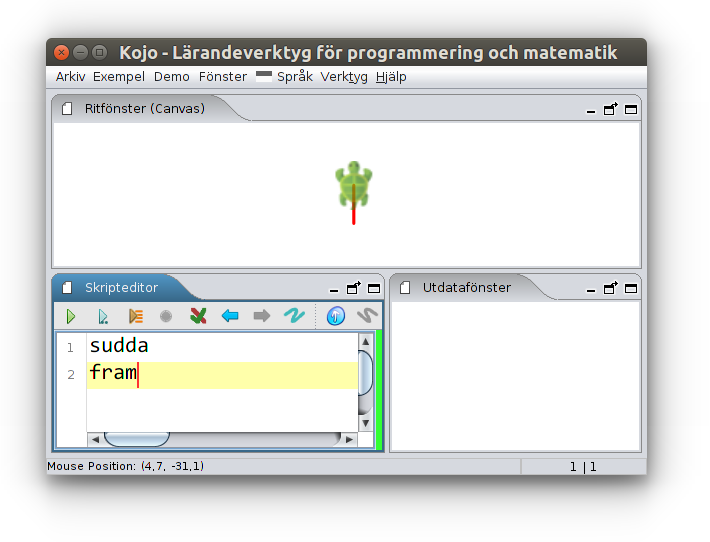
\includegraphics[width=14cm]{../img/kojo.png}

\end{multicols}

\chapter{Ditt första program}
\begin{multicols}{2}
\section*{\color{MidnightBlue}Du lär dig:}
Skriva kod i en editor.\\
Köra igång ett program.
\section*{\color{MidnightBlue}Uppdrag:}
Skriv detta program i editorn:

\begin{lstlisting}[basicstyle={\ttfamily\fontsize{24}{24}\selectfont}]
sudda
fram
\end{lstlisting}
        
Tryck på den gröna play-knappen\\
för att köra igång ditt program.

\columnbreak

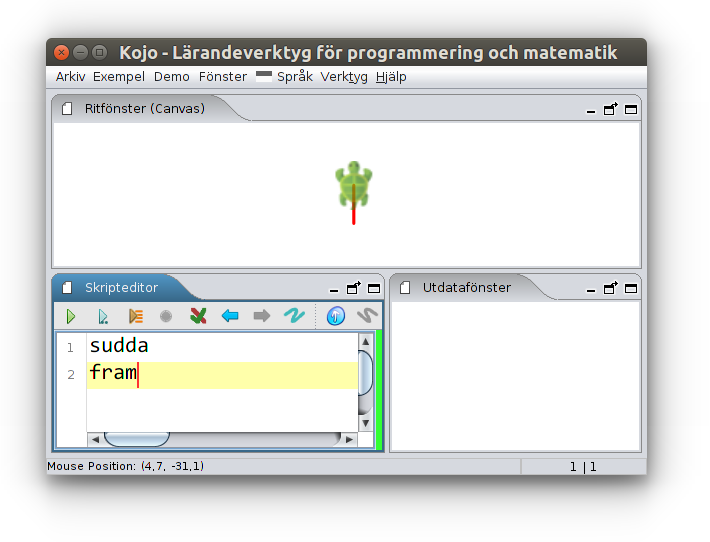
\includegraphics[width=14cm]{../img/fram.png}
\end{multicols}

\chapter{Rita en kvadrat}
\begin{multicols}{2}
\section*{\color{MidnightBlue}Du lär dig:}
Att satser i sekvens körs i tur och ordning.\\
Att ordningen spelar stor roll.
\section*{\color{MidnightBlue}Uppdrag:}
Skriv in och utöka detta program så att paddan ritar en kvadrat:

\begin{lstlisting}[basicstyle={\ttfamily\fontsize{24}{24}\selectfont}]
sudda
fram
höger
\end{lstlisting}
        

\columnbreak

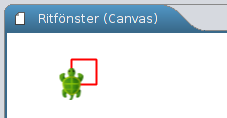
\includegraphics[width=14cm]{../img/kvadrat.png}
\end{multicols}



\end{document}
